\documentclass[12pt]{article}
\usepackage[a4paper, total={16cm,25cm}]{geometry}
\usepackage{titlesec}
\usepackage{graphicx}
\usepackage{float}
\PassOptionsToPackage{hyphens}{url}\usepackage{hyperref}
\usepackage{fancyhdr}
\setlength{\headheight}{30pt}
\pagestyle{fancy}
\fancyhead[L]{HSI使用說明書}
\fancyhead[R]{\leftmark}
\renewcommand{\headrulewidth}{0pt}
\usepackage{amsmath}
\usepackage{latexsym}
\usepackage{multirow}
\graphicspath{ {./images/} }
\usepackage[backend=biber, citestyle=numeric, bibstyle=numeric, sorting=none]{biblatex}
\addbibresource{ref.bib}
\usepackage{mathspec}   %加這個就可以設定字體
\usepackage{xeCJK}       %讓中英文字體分開設置
\setCJKmainfont{Noto Serif CJK TC} %設定中文為系統上的字型
\newCJKfontfamily[chineseSans]\CJKsans{Noto Sans CJK TC}
\setmainfont{Roboto Serif}
\setsansfont{Roboto}
\setmonofont{Roboto Mono}
\XeTeXlinebreaklocale "zh"             %這兩行一定要加,中文才能自動換行
\XeTeXlinebreakskip = 0pt plus 1pt     %這兩行一定要加,中文才能自動換行
\renewcommand{\baselinestretch}{1.35}
\renewcommand{\figurename}{圖}
\renewcommand{\tablename}{表}
\renewcommand{\abstractname}{摘要}
\renewcommand{\contentsname}{目錄}
\renewcommand{\listtablename}{表格目錄}
%\renewcommand*{\bibfont}{\footnotesize}
\titleformat*{\section}{\Large \bfseries}
\titleformat*{\subsection}{\large \bfseries}
\titleformat*{\subsubsection}{\bfseries}

\begin{document}
    \thispagestyle{empty}\noindent{\Large HyperSpectral Imaging System}\newline
    {\large 軟體操作使用說明書}\newpage
    \tableofcontents\newpage
    \section{啟動軟體}
    本軟體尚未編譯為可執行檔,請開啟並執行HIS.lvproj中的main.vi,即可啟動軟體。軟體啟動時,會自動偵測是否能成功連接iXon相機,若連接失敗,系統判定並未連接iXon,則軟體會出現訊息視窗,
    並自動進入讀取模式。
    
    一旦軟體啟動,並成功連接iXon,系統即會自動開啟iXon的TE Cooler,此時使用者即可自行輸入欲達到的溫度,待系統完成降溫且溫度穩定後,Cooler燈號才會轉為綠色。
    當系統硬體都成功連接後,軟體會自動進入影像與掃描設定的模式。此時在畫面左半側的系統控制區,多數的控制元件都會啟動,少數呈現刷白的控制元件是無法使用的。此時可以對系統的影像、掃描參數進行設定,
    為掃描進行準備。

    同時,在畫面的右半側,共計有四個顯示螢幕,是軟體的影像資料檢索介面。該介面此時也是處於啟動狀態,能夠幫助使用者檢視當前設定下的影像資料。
    \begin{figure}[h]
        \centering
        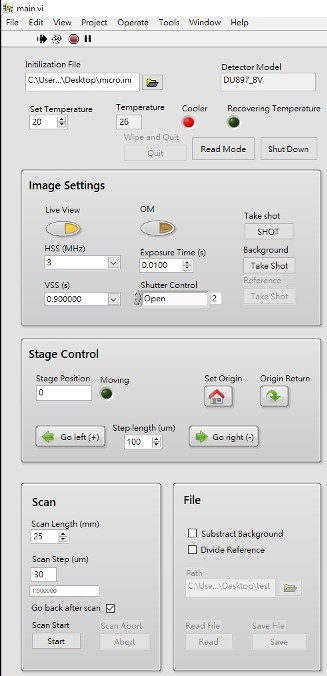
\includegraphics[width=0.33\linewidth]{settingPanel.jpeg}
        \caption{系統控制區。}
    \end{figure}
    \begin{figure}[h]
        \centering
        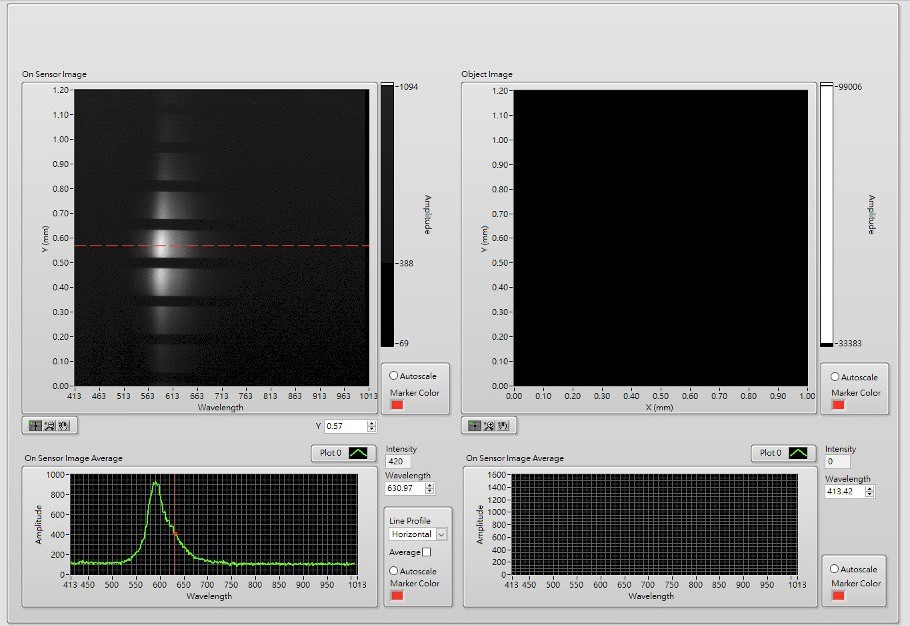
\includegraphics[width=0.75\linewidth]{browsePanel.jpeg}
        \caption{影像資料檢索介面。}
    \end{figure}

    \section{系統控制區}
    \subsection{啟動與模式控制區}
    在本區中選取系統起始參數檔(init file),一般來說使用者不需特別理會起始參數檔。若要切換起始參數檔,必須將軟體關閉後,重新指定參數檔路徑,再開啟軟體。

    若系統啟動後成功連接iXon,本區也會顯示出iXon的型號。
    \subsection{影像設定區}
    \subsection{載台控制區}
    \subsection{掃描設定區}
    \subsection{資料檢索區}

\end{document}